% Drawing 154/03-2 -- folder 154, batch 03, archive page 43 (PDF page 44).
% Transcription: figures dans la colonne de droite, marquées a), b), c) : a) une droite verte traversée par un trait orange ; b) un segment vert aux extrémités fourchues, traversé en son milieu par une étoile de traits orange ; c) une croix verte traversée d'une croix orange
% Kind: three local pictures a), b), c). Method 2 (schematic redraw from the facsimile). Status: ok.
% Notes: Right column: a) a green segment with end ticks crossed by an orange stroke (the label reads like « -) » on the facsimile); b) a green segment with forked ends, crossed in its middle by a star of three orange strokes; c) a green cross crossed by an orange cross. The order on the page is b) on top, a) in the middle, c) at the bottom.
% Coordinates: 1 unit = 1 mm = 1/100 of the crop width (bbox in page fractions: [0.669, 0.403, 0.864, 0.502]).
% Redrawn by Claude (claude-opus-5-5), issue #73, 2026-11-07; not checked by a human; not compiled (no TeX in the session).
% Rights: reproduces part of the work -- behind RENDER_TRANSCRIPTS, never published by itself.
\documentclass[tikz,border=3pt]{standalone}
\usepackage{amsmath,amssymb}
\usetikzlibrary{patterns,arrows.meta}
\tikzset{Or/.style={orange!90!black}, Ye/.style={yellow!80!orange}, Lg/.style={green!60!black!70}, Dg/.style={green!45!black}, Br/.style={brown!80!black}, Rd/.style={red!85!black}, Bl/.style={blue!70!black}, Gy/.style={black!40}, pencil/.style={black!45}, struck/.style={black!35}, mark/.style={circle,draw,inner sep=1.3pt}, pt/.style={circle,fill,inner sep=0.9pt}, opt/.style={circle,draw,fill=white,inner sep=1.1pt}}
\begin{document}
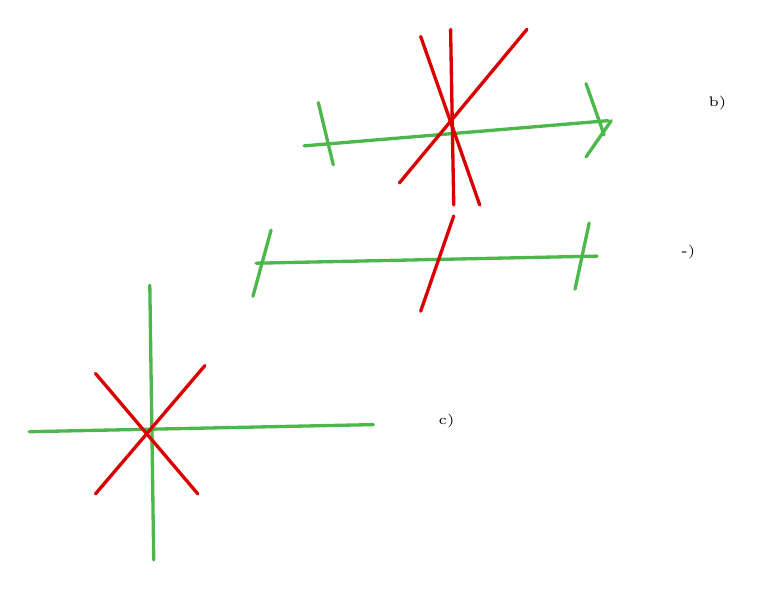
\begin{tikzpicture}[x=1mm,y=1mm,line cap=round,line join=round,font=\scriptsize]
\draw[Lg,very thick] (40.5,-19.5) -- (79.1,-16.3);
\draw[Lg,very thick] (42.3,-14) -- (44.2,-21.9);
\draw[Lg,very thick] (76.3,-11.6) -- (78.6,-18.1);
\draw[Lg,very thick] (79.5,-16.3) -- (76.3,-20.9);
\draw[Rd,very thick] (55.3,-5.6) -- (62.8,-27);
\draw[Rd,very thick] (68.8,-4.7) -- (52.6,-24.2);
\draw[Rd,very thick] (59.1,-4.7) -- (59.5,-27);
\node[inner sep=1pt] at (93,-14) {\tiny b)};
\draw[Lg,very thick] (34.4,-34.4) -- (77.7,-33.5);
\draw[Lg,very thick] (36.3,-30.2) -- (34,-38.6);
\draw[Lg,very thick] (76.7,-29.3) -- (74.9,-37.7);
\draw[Rd,very thick] (59.5,-28.4) -- (55.3,-40.5);
\node[inner sep=1pt] at (89.3,-33) {\tiny -)};
\draw[Lg,very thick] (5.6,-55.8) -- (49.3,-54.9);
\draw[Lg,very thick] (20.9,-37.2) -- (21.4,-72.1);
\draw[Rd,very thick] (14,-48.4) -- (27,-63.7);
\draw[Rd,very thick] (27.9,-47.4) -- (14,-63.7);
\node[inner sep=1pt] at (58.6,-54.4) {\tiny c)};
\end{tikzpicture}
\end{document}
